\documentclass[10pt,aspectratio=169]{ntuabeamer}

\graphicspath{{assets/}}

\framesource{sandia2014}{Kalashnikova et al.\ \href{https://www.osti.gov/biblio/1177206}{\emph{Reduced Order Modeling for Prediction and Control of Large-Scale Systems}}. Sandia Report SAND2014-4693, 2014.}
\framesource{bai2021}{Bai~Z., Peng~L. \href{https://doi.org/10.1186/s40323-021-00213-5}{\emph{Non-intrusive nonlinear model reduction via machine learning approximations to low-dimensional operators}}. Adv.\ Model.\ Simul.\ Eng.\ Sci., 2021.}
\framesource{kutz2016}{Kutz, Brunton, Brunton, Proctor. \href{https://epubs.siam.org/doi/book/10.1137/1.9781611974508}{\emph{Dynamic Mode Decomposition: Data-Driven Modeling of Complex Systems}}. SIAM, 2016.}

\title{Principal Component Analysis and Reduced-Order Modeling}
\subtitle{Reduced-order modeling motivation, workflow, and principal component analysis as a concrete construction}
\author{NTUA School of Civil Engineering}
\date{\today}

\begin{document}

\begin{frame}[plain]
  \makepresentationtitle
\end{frame}

\sectiondivider{Reduced-Order Modeling (ROM) Context}

\begin{frame}{Why Reduced-Order Modeling?}
  \small
  Many scientific computing tasks are \textcolor{ntuablue}{many-query problems}: we solve the same partial differential equation (PDE) repeatedly for different parameters, loads, boundary conditions, or geometries.

  \[
    \mathcal{R}\!\left(\bd{u}(\xi); \xi\right) = 0,
    \qquad \xi \in \mathcal{P}
  \]

  \begin{itemize}
    \item \(\xi\): parameter vector describing one query
    \item \(\mathcal{P}\): parameter domain
    \item \(\bd{u}(\xi) \in \mathbb{R}^{D}\): discretized high-fidelity state
    \item \(\mathcal{R}(\cdot;\xi)\): PDE residual operator
    \item \(D\): dimension of the high-fidelity model
  \end{itemize}
\end{frame}

\begin{frame}{What a Reduced-Order Model Does}
  \small
  A reduced-order model (ROM) replaces the high-dimensional state by a low-dimensional state and a reconstruction map:

  \[
    \bd{u}_r(\xi)\in\mathbb{R}^{r},
    \qquad
    \widehat{\bd{u}}(\xi)=\mathrm{Dec}_r\!\left(\bd{u}_r(\xi);\xi\right),
    \qquad
    r \ll D
  \]

  \begin{itemize}
    \item \(\bd{u}_r(\xi)\): reduced state
    \item \(\mathrm{Enc}_r\): encoder map \((\mathbb{R}^D\to\mathbb{R}^r)\)
    \item \(\mathrm{Dec}_r\): decoder / reconstruction map \((\mathbb{R}^r\to\mathbb{R}^D)\);
          may depend on \(\xi\) for general ROMs --- the PCA decoder does not
    \item \(r\): reduced dimension
  \end{itemize}

  \vspace{0.3em}
  \textcolor{ntuablue}{ROM types}
  \begin{itemize}
    \item Projection ROMs are usually \emph{intrusive} (require access to system operators,
          e.g.\ \(\bd{K}(\xi)\))\framecite{bai2021}
    \item Non-intrusive ROMs also exist\framecite{bai2021}
  \end{itemize}
\end{frame}

\begin{frame}{High-Level Workflow}
  \small
  \(N_{\mathrm{tot}} = N_{\mathrm{train}} + N_{\mathrm{deploy}}\) queries drawn from \(\mathcal{P}\)
  (\(N_{\mathrm{deploy}}\): number of online deployment queries).

  \threecols
  {
    \textcolor{ntuablue}{Offline — data}
    \begin{itemize}
      \item Sample \(\{\xi_j\}_{j=1}^{N_{\mathrm{train}}}\subset\mathcal{P}\)
      \item \textbf{High-fidelity solve}: \(\mathcal{R}(\bd{u}(\xi_j);\xi_j)=0\)
      \item Store high-fidelity snapshots \(\bd{u}(\xi_j)\in\mathbb{R}^D\)
    \end{itemize}
  }
  {
    \textcolor{ntuablue}{Offline — model}
    \begin{itemize}
      \item Build reduced basis \((r\ll D)\)
      \item Form \(\mathrm{Enc}_r,\,\mathrm{Dec}_r\)
      \item Assemble reduced model
    \end{itemize}
  }
  {
    \textcolor{ntuablue}{Online — deploy}
    \begin{itemize}
      \item Query \(\xi_i\in\mathcal{P}\), \(i=1,\dots,N_{\mathrm{deploy}}\)
      \item Solve reduced model in \(\mathbb{R}^r\)
      \item Reconstruct \(\widehat{\bd{u}}(\xi_i)=\mathrm{Dec}_r(\bd{u}_r(\xi_i))\)
    \end{itemize}
  }
\end{frame}

\begin{frame}{When Does ROM Actually Pay Off?\framecite{sandia2014}}
  \small
  Let
  \[
    T_{\mathrm{off}} = T_{\mathrm{snap}} + T_{\mathrm{build}}
  \]
  denote the \textcolor{ntuablue}{total offline time} (\(T\): total, \(t\): per query):
  \begin{itemize}
    \item \(T_{\mathrm{snap}} = N_{\mathrm{train}}\,t_{\mathrm{HF}}\): total time for all \(N_{\mathrm{train}}\) high-fidelity solves
    \item \(T_{\mathrm{build}}\): total time to build the reduced basis and reduced model
  \end{itemize}

  \vspace{0.3em}
  A compact break-even estimate is
  \[
    N_{\mathrm{use}}
    >
    \frac{T_{\mathrm{off}}}
         {t_{\mathrm{HF}} - t_{\mathrm{ROM}}}
  \]

  \begin{itemize}
    \item \(t_{\mathrm{HF}}\): time per high-fidelity solve
    \item \(t_{\mathrm{ROM}}\): time per ROM solve \((\ll t_{\mathrm{HF}})\)
    \item \(N_{\mathrm{use}}\): minimum deployment queries for ROM to recoup its offline cost
  \end{itemize}
\end{frame}

\sectiondivider{Principal Component Analysis (PCA) Theory}

\begin{frame}{PCA Snapshot Basis\framecite{kutz2016}}
  \small
  In the ROM literature, this same construction is often called
  \textcolor{ntuablue}{proper orthogonal decomposition (POD)}.
  Here we keep the term \textcolor{ntuablue}{principal component analysis (PCA)}.

  \[
    \bar{\bd{u}}
    =
    \frac{1}{N_{\mathrm{train}}}
    \sum_{j=1}^{N_{\mathrm{train}}}
    \bd{u}(\xi_j),
    \qquad
    \bd{U}
    =
    \begin{bmatrix}
      \bd{u}(\xi_1)^{\top} \\
      \vdots \\
      \bd{u}(\xi_{N_{\mathrm{train}}})^{\top}
    \end{bmatrix}
    \in \mathbb{R}^{N_{\mathrm{train}} \times D}
  \]
  \[
    \bd{U}_c = \bd{U} - \mathbf{1}\bar{\bd{u}}^{\top},
    \qquad
    (\bd{U}_c)_{j,:} = (\bd{u}(\xi_j)-\bar{\bd{u}})^{\top}
    \quad\text{(centered snapshot matrix)}
  \]

  \begin{itemize}
    \item \(\bar{\bd{u}} \in \mathbb{R}^{D}\): mean high-fidelity state
    \item \(\bd{U}\): high-fidelity snapshot matrix; \(\bd{U}_c\): mean-centered
    \item PCA extracts the reduced basis from \(\bd{U}_c\)
  \end{itemize}
\end{frame}

\begin{frame}{PCA Intuition}
  \begin{figure}
    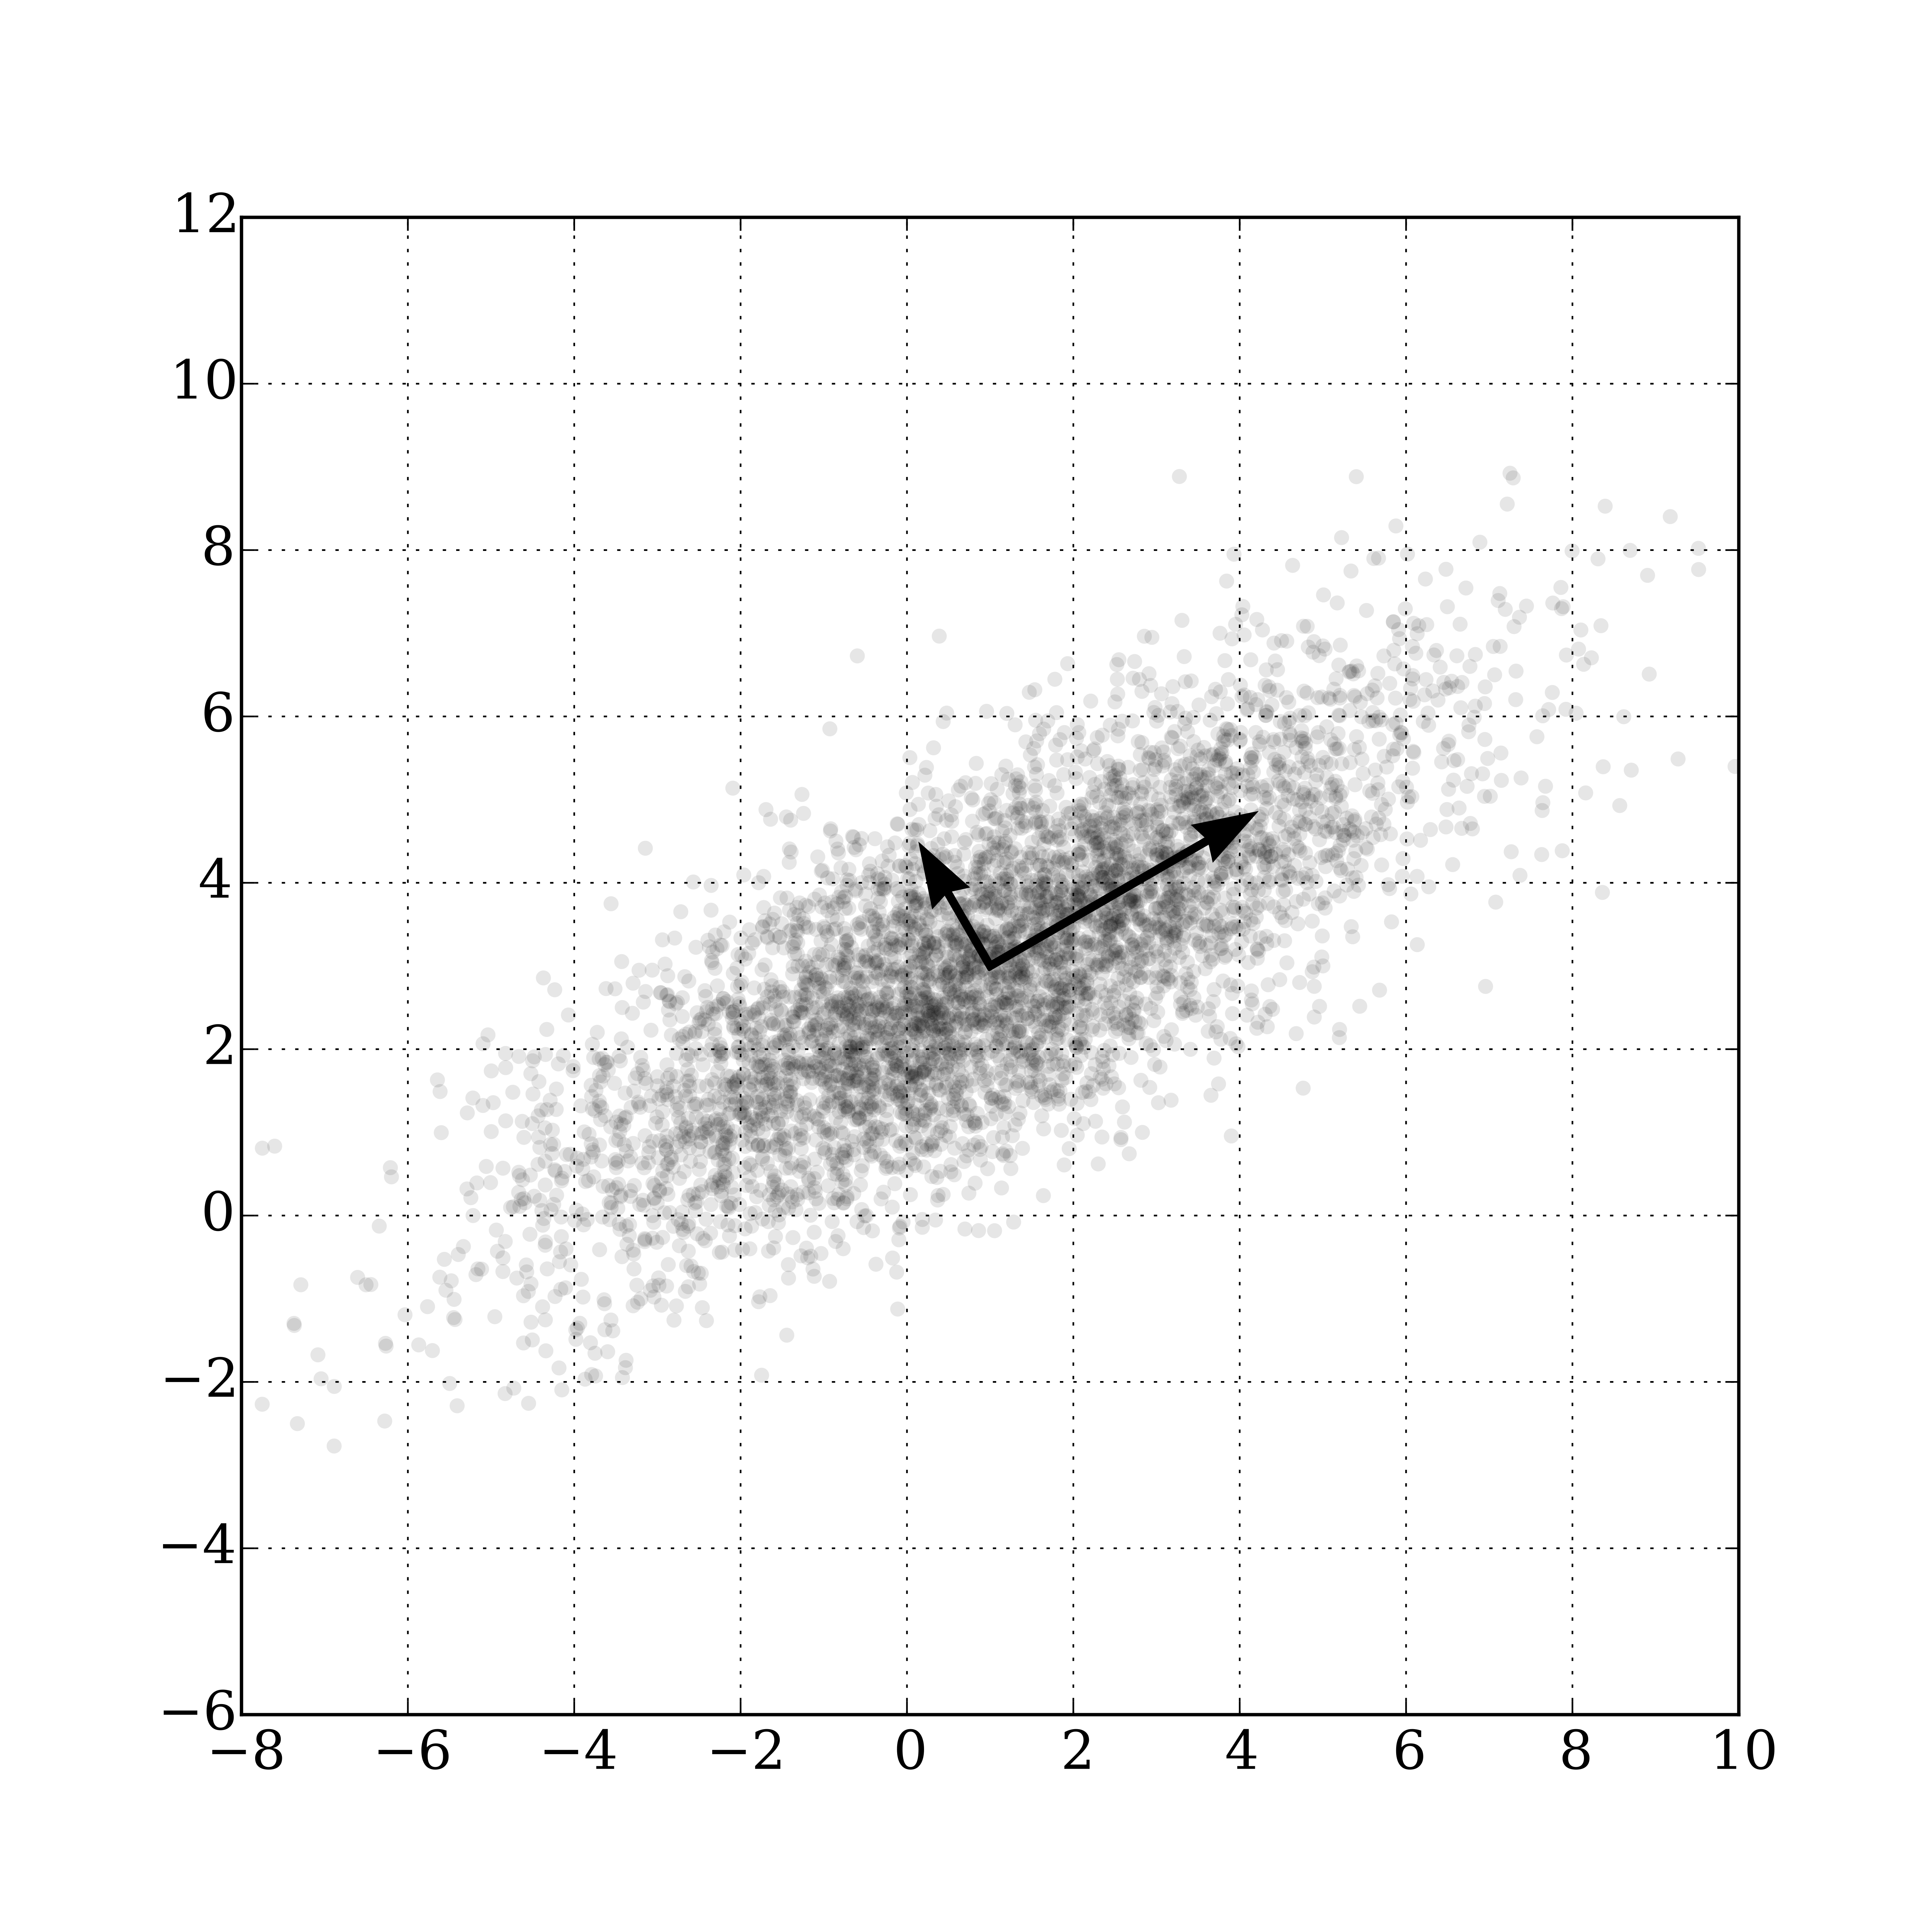
\includegraphics[width=0.9\textwidth,height=0.66\textheight,keepaspectratio]{principal-axes.png}
    \caption{\footnotesize Each snapshot \(\bd{u}(\xi_j)\) is a point in \(\mathbb{R}^D\).
      When snapshots cluster near a low-dimensional subspace, PCA identifies that subspace
      as the span of the leading principal axes (shown as arrows).}
  \end{figure}
\end{frame}

\begin{frame}{PCA Basis Construction}
  \small
  \[
    \bd{C}=\frac{1}{N_{\mathrm{train}}}\bd{U}_c^{\top}\bd{U}_c\in\mathbb{R}^{D\times D},
    \qquad
    \bd{C}\bd{v}_i=\lambda_i\bd{v}_i
  \]
  \(\bd{C}\) is symmetric positive semidefinite; its eigenvectors are orthonormal and solve
  \[
    \max_{\|\bd{v}\|=1}\;\mathrm{Var}(\bd{U}_c\bd{v})
    =
    \max_{\|\bd{v}\|=1}\;\bd{v}^{\top}\bd{C}\bd{v}
    \quad\text{(zero mean since \(\bd{U}_c\) is centred)}.
  \]
  Along axis \(\bd{v}_i\) the eigenvalue \(\lambda_i\) equals the captured variance.
  Denoting by \(\sigma_i\) the \(i\)-th \textcolor{ntuablue}{singular value} of \(\bd{U}_c\):
  \[
    \lambda_i = \frac{\sigma_i^2}{N_{\mathrm{train}}}
  \]
  because \(\bd{C}=\tfrac{1}{N_{\mathrm{train}}}\bd{U}_c^{\top}\bd{U}_c\) and \(\bd{U}_c^{\top}\bd{U}_c=\bd{V}\,\bd{\Sigma}^{\top}\bd{\Sigma}\,\bd{V}^{\top}\) from the SVD (see appendix).

  \begin{itemize}
    \item Reduced basis: \(\bd{V}_r = [\bd{v}_1,\dots,\bd{v}_r]\in\mathbb{R}^{D\times r}\),\quad \(\bd{V}_r^{\top}\bd{V}_r = \bd{I}_r\)
    \item \(\mathrm{Enc}_r\) \((\mathbb{R}^D\to\mathbb{R}^r)\): \(\bd{u}_r=\bd{V}_r^{\top}(\bd{u}-\bar{\bd{u}})\)
    \item \(\mathrm{Dec}_r\) \((\mathbb{R}^r\to\mathbb{R}^D)\): \(\widehat{\bd{u}}=\bar{\bd{u}}+\bd{V}_r\bd{u}_r\)
  \end{itemize}
\end{frame}

\begin{frame}{Eigenvalue Decay}
  \small
  Ordered \(\lambda_1\geq\lambda_2\geq\cdots\geq\lambda_{D}\geq 0\)
  (at most \(D\) nonzero);
  leading modes capture the dominant variability.

  \begin{figure}
    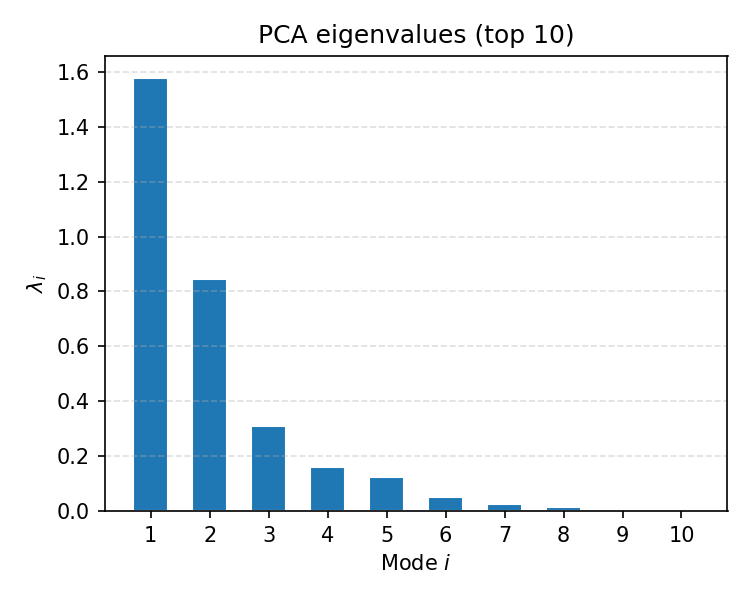
\includegraphics[width=\textwidth,height=0.58\textheight,keepaspectratio]{eigenvalues.png}
    \caption{\footnotesize Descending PCA eigenvalues rank the principal directions by captured variance.}
  \end{figure}
\end{frame}

\begin{frame}{Choosing the Reduced Dimension \(r\)}
  \small
  \twocols[0.45\textwidth][0.51\textwidth]
  {
    A common truncation criterion is the
    \textcolor{ntuablue}{cumulative explained variance}
    \[
      \eta(r)
      =
      \frac{\sum_{i=1}^{r} \lambda_i}
           {\sum_{i=1}^{D} \lambda_i}
    \]
    fraction of variance in the first \(r\) modes.
    Equivalently in terms of singular values \(\sigma_i\):
    \[
      \eta(r) = \frac{\sum_{i=1}^{r}\sigma_i^2}{\sum_{i=1}^{D}\sigma_i^2}
    \]
    (at most \(D\) terms nonzero).

    \begin{itemize}
      \item Choose smallest \(r\) with \(\eta(r)\geq\) target
      \item \(1-\eta(r)\): information loss
    \end{itemize}
  }
  {
    \begin{figure}
      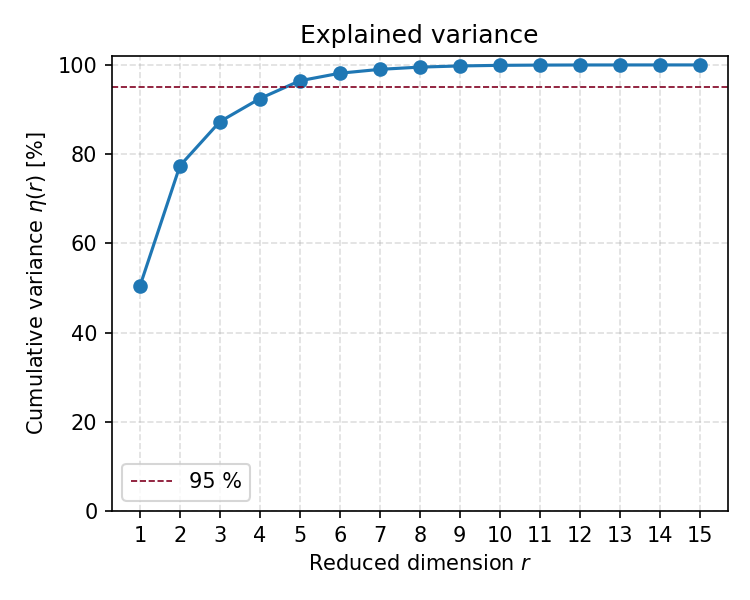
\includegraphics[width=\textwidth,height=0.55\textheight,keepaspectratio]{explained-variance.png}
      \caption{\footnotesize Cumulative explained variance.}
    \end{figure}
  }

  \vspace{0.2em}
  \textcolor{ntuablue}{Note:} the denominator is the \textbf{total variance}
  \(\sum_{i=1}^{D}\lambda_i = \mathrm{tr}(\bd{C})\),
  obtainable directly from the diagonal of \(\bd{C}\) --- no full eigendecomposition required.
\end{frame}

\sectiondivider{PCA-Galerkin Example}

\begin{frame}{PCA-ROM: Approximation Ansatz}
  \small
  \textcolor{ntuablue}{High-fidelity system} \((\mathbb{R}^D)\):
  \[
    \bd{K}(\xi)\bd{u}(\xi) = \bd{f}(\xi),
    \qquad
    \bd{K}(\xi)\in\mathbb{R}^{D\times D},
    \quad
    \bd{u}(\xi),\bd{f}(\xi)\in\mathbb{R}^{D}
  \]
  with PCA objects \(\bar{\bd{u}}\in\mathbb{R}^{D}\), \(\bd{V}_r\in\mathbb{R}^{D\times r}\), \(\bd{V}_r^{\top}\bd{V}_r=\bd{I}_r\).

  \vspace{0.4em}
  \textcolor{ntuablue}{Decode} into the original system
  \((\bd{u}_r\in\mathbb{R}^r \;\to\; \widehat{\bd{u}}\in\mathbb{R}^D)\):
  \[
    \bd{u}(\xi)\approx\widehat{\bd{u}}(\xi)=\bar{\bd{u}}+\bd{V}_r\bd{u}_r(\xi)
    \quad\Rightarrow\quad
    \bd{K}(\xi)\bigl(\bar{\bd{u}}+\bd{V}_r\bd{u}_r(\xi)\bigr) = \bd{f}(\xi)
  \]

  \textcolor{ntuablue}{Centered form} (still \(\mathbb{R}^D\), move mean response to RHS):
  \[
    \bd{K}(\xi)\bd{V}_r\bd{u}_r(\xi)
    =
    \underbrace{\bd{f}(\xi)-\bd{K}(\xi)\bar{\bd{u}}}_{\text{modified RHS}\,\in\mathbb{R}^D}.
  \]

  Overdetermined (\(D\) equations, \(r\) unknowns); closed by Galerkin projection \(\to\mathbb{R}^r\).
\end{frame}

\begin{frame}{PCA-ROM: Galerkin Projection}
  \small
  \textcolor{ntuablue}{Project} \((\mathbb{R}^D\to\mathbb{R}^r)\): residual
  \(\bd{r}=\bd{K}(\xi)\bd{V}_r\bd{u}_r-\bigl(\bd{f}(\xi)-\bd{K}(\xi)\bar{\bd{u}}\bigr)\in\mathbb{R}^D\)
  must be \(\bd{V}_r\)-orthogonal:
  \[
    \bd{V}_r^{\top}\,\underbrace{
      \left(
        \bd{K}(\xi)\bd{V}_r\bd{u}_r(\xi)
        -
        \bigl(\bd{f}(\xi)-\bd{K}(\xi)\bar{\bd{u}}\bigr)
      \right)
    }_{\bd{r}\,\in\,\mathbb{R}^D}
    =
    \bd{0}.
  \]

  \textcolor{ntuablue}{Reduced coordinates} \((\mathbb{R}^r)\) — define reduced operators:
  \[
    \bd{K}_r(\xi) = \bd{V}_r^{\top}\bd{K}(\xi)\bd{V}_r \in\mathbb{R}^{r\times r},
    \qquad
    \bd{f}_r(\xi) = \bd{V}_r^{\top}\!\left(\bd{f}(\xi) - \bd{K}(\xi)\bar{\bd{u}}\right)\in\mathbb{R}^r.
  \]
  \[
    \bd{K}_r(\xi)\bd{u}_r(\xi) = \bd{f}_r(\xi).
    \qquad\textcolor{gray}{\text{(solve in }\mathbb{R}^r\text{)}}
  \]

  \textcolor{ntuablue}{Decode} \((\mathbb{R}^r\to\mathbb{R}^D)\):
  \[
    \widehat{\bd{u}}(\xi)=\mathrm{Dec}_r(\bd{u}_r(\xi))=\bar{\bd{u}}+\bd{V}_r\bd{u}_r(\xi).
  \]
\end{frame}

\begin{frame}{PCA-Galerkin Algorithm}
  \small
  \begin{enumerate}
    \item High-fidelity solves, for \(j=1,\dots,N_{\mathrm{train}}\):
    \[
      \bd{K}(\xi_j)\bd{u}(\xi_j)=\bd{f}(\xi_j),
    \]
    \item Mean and centered snapshots \textcolor{gray}{(\(\mathrm{Enc}_r\))}:
    \[
      \bar{\bd{u}}=\frac{1}{N_{\mathrm{train}}}\sum_{j=1}^{N_{\mathrm{train}}}\bd{u}(\xi_j),
      \qquad
      (\bd{U}_c)_{j,:}=(\bd{u}(\xi_j)-\bar{\bd{u}})^{\top}.
    \]
    \item PCA basis:
    \[
      \bd{C}=\frac{1}{N_{\mathrm{train}}}\bd{U}_c^{\top}\bd{U}_c,
      \qquad
      \bd{C}\bd{v}_i=\lambda_i\bd{v}_i,
      \qquad
      \bd{V}_r=[\bd{v}_1,\dots,\bd{v}_r].
    \]
    \item Reduced operators:
    \[
      \bd{K}_r(\xi)=\bd{V}_r^{\top}\bd{K}(\xi)\bd{V}_r,
      \qquad
      \bd{f}_r(\xi)=\bd{V}_r^{\top}\!\left(\bd{f}(\xi)-\bd{K}(\xi)\bar{\bd{u}}\right).
    \]
    \item Deploy, for \(i=1,\dots,N_{\mathrm{deploy}}\)
          \textcolor{gray}{(solve \(\to\) \(\mathrm{Dec}_r\))}:
    \[
      \bd{K}_r(\xi_i)\bd{u}_r(\xi_i)=\bd{f}_r(\xi_i),
      \qquad
      \widehat{\bd{u}}(\xi_i)=\mathrm{Dec}_r(\bd{u}_r(\xi_i))=\bar{\bd{u}}+\bd{V}_r\bd{u}_r(\xi_i).
    \]
  \end{enumerate}
\end{frame}

\begin{frame}{MRE: Snapshot Spaces}
  \small
  Minimal example: \(D=3\), \(r=2\), \(N_{\mathrm{train}}=N_{\mathrm{deploy}}=200\),
  \(\xi=(\xi_1,\xi_2)\sim\mathrm{Uniform}([0,3]\times[0,2])\),
  system \(\bd{K}(\xi_1)\bd{u}=\bd{f}(\xi_1,\xi_2)\) with tridiagonal \(\bd{K}\).

  \twocols[0.48\textwidth][0.48\textwidth]
  {
    \begin{figure}
      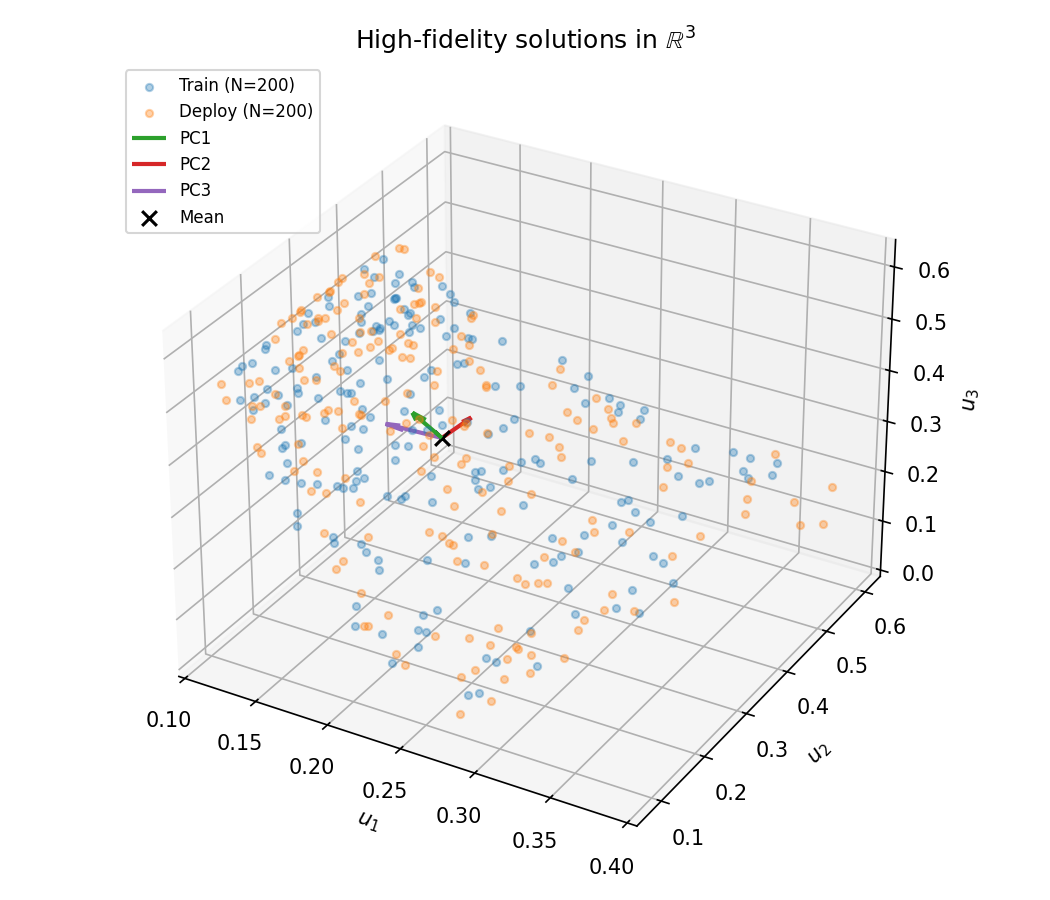
\includegraphics[width=\textwidth,height=0.50\textheight,keepaspectratio]{3d-original-space.png}
      \caption{\footnotesize All snapshots in \(\mathbb{R}^3\)
        (\textcolor{ntuablue}{blue}: train,
         \textcolor{orange}{orange}: deploy).
        Arrows: first two PC axes from \(\bar{\bd{u}}\).}
    \end{figure}
  }
  {
    \begin{figure}
      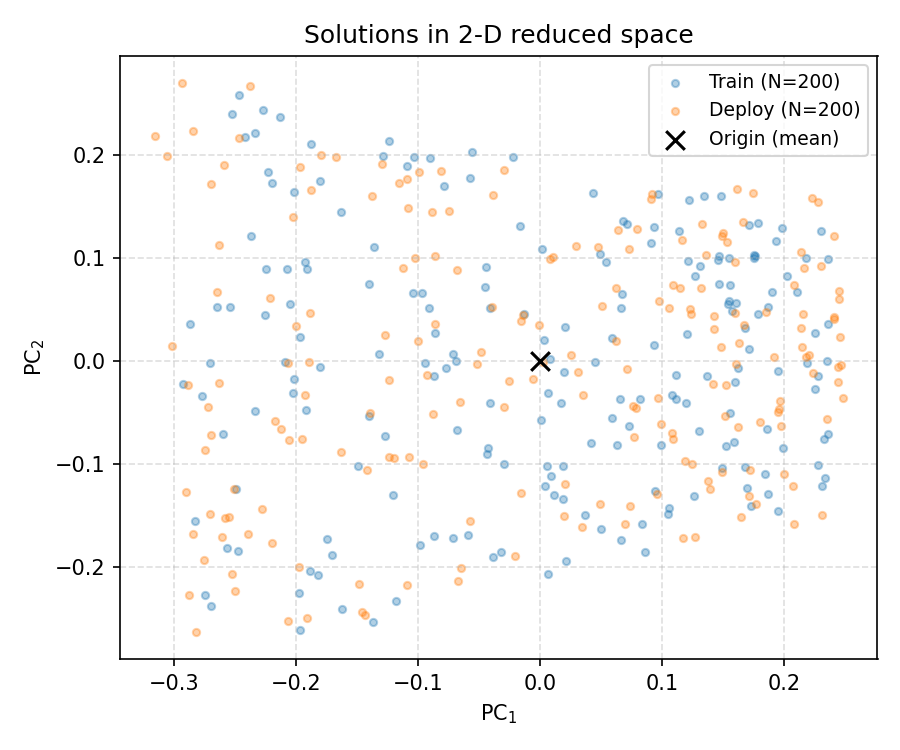
\includegraphics[width=\textwidth,height=0.50\textheight,keepaspectratio]{2d-reduced-space.png}
      \caption{\footnotesize Same snapshots encoded to \(\mathbb{R}^2\)
        via \(\bd{u}_r = \bd{V}_r^{\top}(\bd{u}-\bar{\bd{u}})\).
        Origin \(=\) mean \(\bar{\bd{u}}\).}
    \end{figure}
  }
\end{frame}

\sectiondivider{Appendix}

\begin{frame}{Appendix: PCA via Covariance or SVD}
  \small
  Starting from the centered snapshot matrix
  \[
    \bd{U}_c \in \mathbb{R}^{N_{\mathrm{train}} \times D},
    \qquad
    \bd{C} = \frac{1}{N_{\mathrm{train}}}\bd{U}_c^{\top}\bd{U}_c \in \mathbb{R}^{D\times D},
  \]
  the PCA eigenproblem is
  \[
    \bd{C}\bd{v}_i = \lambda_i \bd{v}_i.
  \]

  The singular value decomposition (SVD) of the same matrix is
  \[
    \bd{U}_c = \bd{W}\bd{\Sigma}\bd{V}^{\top}.
  \]

  \begin{itemize}
    \item \(\bd{W} \in \mathbb{R}^{N_{\mathrm{train}} \times N_{\mathrm{train}}}\): left singular vectors, acting on the sample side
    \item \(\bd{\Sigma} \in \mathbb{R}^{N_{\mathrm{train}} \times D}\): rectangular diagonal matrix, \(\Sigma_{ii}=\sigma_i\)
    \item \(\bd{V} \in \mathbb{R}^{D \times D}\): right singular vectors, acting on the state/feature side
  \end{itemize}

  \textcolor{gray}{\footnotesize In practice the economy (thin) SVD is used:
    \(\bd{W}\in\mathbb{R}^{N_{\mathrm{train}}\times k}\),
    \(\bd{\Sigma}\in\mathbb{R}^{k\times k}\),
    \(k=\min(N_{\mathrm{train}},D)\).}

  Therefore (\(\bd{\Sigma}^{\top}\bd{\Sigma}=\mathrm{diag}(\sigma_i^2)\in\mathbb{R}^{D\times D}\)):
  \[
    \bd{U}_c^{\top}\bd{U}_c = \bd{V}\,\bd{\Sigma}^{\top}\bd{\Sigma}\,\bd{V}^{\top},
  \]
  so the PCA eigenvectors are the right singular vectors:
  \(\bd{v}_i = \text{column } i \text{ of } \bd{V}.\)
\end{frame}

\begin{frame}{Appendix: Relationship Between Eigenvalues}
  \small
  Since
  \[
    \bd{C} = \frac{1}{N_{\mathrm{train}}}\bd{U}_c^{\top}\bd{U}_c
    = \frac{1}{N_{\mathrm{train}}}\bd{V}\,\bd{\Sigma}^{\top}\bd{\Sigma}\,\bd{V}^{\top},
  \]
  the PCA eigenvalues and SVD singular values satisfy
  \[
    \lambda_i = \frac{\sigma_i^2}{N_{\mathrm{train}}}.
  \]

  If we instead diagonalize the smaller Gram matrix,
  \[
    \bd{G} = \frac{1}{N_{\mathrm{train}}}\bd{U}_c\bd{U}_c^{\top}
    = \frac{1}{N_{\mathrm{train}}}\bd{W}\,\bd{\Sigma}\bd{\Sigma}^{\top}\,\bd{W}^{\top},
  \]
  where \(\bd{G}\) is the sample-side Gram matrix.
  \begin{itemize}
    \item eigenvectors of \(\bd{C}\): right singular vectors \(\bd{V}\)
    \item eigenvectors of \(\bd{G}\): left singular vectors \(\bd{W}\)
    \item same nonzero eigenvalues: \(\lambda_i = \sigma_i^2/N_{\mathrm{train}}\)
    \item if \(N_{\mathrm{train}} \ll D\), solve the sample-side problem
  \end{itemize}
\end{frame}

\end{document}
